\chapter{Desarrollo del Proyecto}
\label{anexo:desarrollo}
En este anexo se documenta el desarrollo por sprints. La planificación y el seguimiento se apoyan en las capturas de DoneTonic y en las horas recogidas en la tabla de revisión. El historial Git permite identificar los cambios técnicos. La actualización se realiza a 17 de noviembre de 2026, conservando las evidencias históricas del Sprint 1 y documentando por separado el cierre del Sprint 2.

\section{Sprint 1: Arquitectura Base}
\subsection{Planificación del sprint 1}
% Objetivo
El objetivo de este bloque es establecer una base de aplicación por capas que conecte la interfaz con la API, la lógica de negocio y la persistencia. El backlog comprende los doce PBI de la Tabla~\ref{tab:revision-sprint1-pbi}, con una estimación conjunta de 40,5 horas. Se agrupan en cuatro hitos: esqueleto y backend; frontend y sesión; persistencia y roles; servicios externos y documentación.
% Fechas
DoneTonic muestra el sprint del 29 de septiembre a las 18:30 al 27 de octubre a las 18:00 de 2026. Las capturas se han obtenido el 27 de octubre y documentan el estado disponible, sin certificar el cierre.
% Sprint backlog con su estimación
Los identificadores P1--P14 se conservan para mantener la trazabilidad. Los saltos de numeración corresponden a los PBI disponibles y no se sustituyen por tareas inventadas. La tabla de revisión recoge las estimaciones y la dedicación introducida para cada PBI.
\begin{center}
\begin{minipage}{\textwidth}
\centering
\includegraphics[width=0.95\textwidth,trim=0 60 0 110,clip]{figs/donetonic-sprint1-planificacion.jpg}
\captionsetup{hypcap=false}
\captionof{figure}{Vista parcial del sprint backlog, capturada el 27 de octubre de 2026. Se muestran sus fechas, la carga asignada de 40,5 horas y 2,5 horas registradas; estas últimas no acreditan toda la dedicación real.}
\label{fig:donetonic-sprint1-backlog}
\end{minipage}
\end{center}

\subsection{Desarrollo del Sprint}
% Problema - Solución
% Lo que no debe ser: un diario del desarrolladors
El primer problema fue separar las reglas de acceso de los detalles de interfaz y almacenamiento. La solución distribuye la presentación en \texttt{cliente/presentacion.js}, las peticiones en \texttt{cliente/rest.js}, las rutas en \texttt{servidor/api.js} y las reglas en \texttt{servidor/logica.js}. El historial del 6 de octubre recoge la gestión de usuarios y la API inicial en memoria.

El segundo problema consistía en conservar el acceso entre peticiones y recargas. Los commits del 9 de octubre incorporan creación e invalidación de sesiones, recuperación de la sesión al recargar y protección de rutas. El registro seguro y el cliente HTTP separado completan este incremento. Las sesiones de esa etapa residían en memoria; su persistencia actual en MongoDB es una mejora del 3 de noviembre.

La pérdida de cuentas al reiniciar se abordó mediante un adaptador de persistencia. El 13 de octubre se incorporó MongoDB y se configuraron Cloud Run y Cloud Build. La configuración externa evita incluir secretos en el código. El 15 de octubre se añadió normalización y validación del correo para evitar variantes inconsistentes de una misma dirección.

Finalmente, el 21 de octubre se incorporó código de confirmación por correo y acceso con Google, junto con un ajuste del entorno de CI para MongoDB. La implementación incluye enlaces de confirmación de un solo uso y el flujo OAuth con PKCE. La existencia del código y de pruebas simuladas no acredita recepción real de correos ni acceso real con Google en producción.

\subsection{Revisión del Sprint}
El incremento permite registrar cuentas, autenticar usuarios, cerrar y recuperar sesiones, aplicar permisos y conservar cuentas en MongoDB. La tabla siguiente relaciona los PBI con sus hitos y horas. Las capturas documentan una situación parcial del tablero a 27 de octubre; no se toma esa fotografía como acta de aceptación final. La validación real de los proveedores externos queda separada de la revisión del código.

La Tabla~\ref{tab:revision-sprint1-pbi} recoge los PBI identificables en las capturas disponibles. La columna Hito relaciona el alcance de cada PBI con los cuatro hitos del enunciado: H1, esqueleto y backend; H2, frontend y sesión; H3, persistencia y roles; H4, servicios externos y cierre. La correspondencia es por contenido y no implica que el PBI se haya trabajado exclusivamente en esa semana.

\begin{center}
\begin{minipage}{\textwidth}
\centering
\small
\renewcommand{\arraystretch}{1.25}
\begin{tabular}{|p{0.07\textwidth}|p{0.36\textwidth}|p{0.15\textwidth}|p{0.13\textwidth}|p{0.12\textwidth}|}
\hline
\textbf{PBI} & \textbf{Descripción} & \textbf{Hito} & \textbf{Estimación (h)} & \textbf{Real (h)} \\ \hline
P1 & Crear repositorio y estructura base. & H1 & 7 & 1 \\ \hline
P2 & Configurar flujo de trabajo y CI/CD. & H1 & 2 & 0,5 \\ \hline
P3 & Configurar entorno y secretos. & H1 y H3 & 1 & 0,5 \\ \hline
P4 & Implementar gestión básica de usuarios. & H1 & 10 & 1,5 \\ \hline
P5 & Implementar eliminación, roles y permisos. & H1 y H3 & 1,5 & 0,5 \\ \hline
P6 & Implementar registro local seguro. & H2 & 2 & 0,5 \\ \hline
P7 & Implementar inicio, cierre y persistencia de sesión. & H2 & 8 & 2 \\ \hline
P9 & Implementar persistencia en base de datos. & H3 & 3 & 1 \\ \hline
P10 & Implementar estructura y comunicación del frontend. & H2 & 1 & 0,5 \\ \hline
P12 & Implementar pruebas automatizadas. & H1 & 2 & 0,5 \\ \hline
P13 & Implementar logging, manejo de errores y documentación. & H3 y H4 & 2 & 1 \\ \hline
P14 & Documentar el sprint 1. & H4 & 1 & 0,5 \\ \hline
\multicolumn{3}{|l|}{\textbf{Total del sprint}} & \textbf{40,5} & \textbf{10,5} \\ \hline
\end{tabular}
\captionsetup{hypcap=false}
\captionof{table}{Revisión del Sprint 1 por PBI: descripción, hito y comparación de horas estimadas y reales.}
\label{tab:revision-sprint1-pbi}
\end{minipage}
\end{center}

\begin{center}
\begin{minipage}{\textwidth}
\centering
\includegraphics[width=0.95\textwidth]{figs/donetonic-sprint1-tablero.jpg}
\captionsetup{hypcap=false}
\captionof{figure}{Vista parcial del tablero el 27 de octubre de 2026, después de revisar los estados: 23 tareas hechas, 3 en curso y 1 pendiente.}
\label{fig:donetonic-sprint1-tablero}
\end{minipage}
\end{center}

\subsection{Retrospectiva}
% Mostrar el Sprint Burndown
% Comentar las horas realizadas y compararlas con lo estimado
El gráfico registra una reducción desde aproximadamente 40,5 unidades estimadas hasta 13, con el último punto visible en el día 15. No se extrapola esa línea hasta el día de captura. El panel informa de un 67\% completado según su estimación de PBI, mientras el tablero muestra un 85\% de tareas hechas (23 de 27): son indicadores distintos. La tabla suma 40,5 horas estimadas y 10,5 horas de dedicación recogida, una diferencia de 30 horas y una relación del 25,9\%. Este resultado se refiere a los valores introducidos en la tabla; no equivale al porcentaje de avance ni demuestra por sí solo una mejora de productividad. El gráfico conserva la unidad de estimación de PBI que muestra DoneTonic.

Como aciertos técnicos destacan la separación por capas, el uso de adaptadores y las pruebas de acceso. Las principales dificultades de seguimiento son la coexistencia de capturas tomadas en momentos distintos y la falta de una comprobación pública de los servicios externos. Como mejora para el siguiente sprint se propone registrar la dedicación al terminar cada tarea y asociar a cada PBI su criterio de aceptación, commit o PR y prueba de revisión. Así se podrá comparar planificación, resultado y esfuerzo con la misma fecha de corte.
\begin{center}
\begin{minipage}{\textwidth}
\centering
\includegraphics[width=0.95\textwidth,trim=25 95 25 184,clip]{figs/donetonic-sprint1-burndown-completo.jpg}
\captionsetup{hypcap=false}
\captionof{figure}{Burndown del sprint 1, capturado el 27 de octubre de 2026. El eje horizontal representa días y el vertical la estimación de PBI; la línea oscura muestra el trabajo restante y el área clara la guía ideal.}
\label{fig:donetonic-sprint1-burndown}
\end{minipage}
\end{center}


\clearpage
\raggedbottom
\section{Sprint 2: gestión del transporte de mobiliario}
\subsection{Planificación y alcance}
El objetivo del segundo incremento es conectar la solicitud del cliente con la revisión administrativa, la planificación desde la base de Yecla y la ejecución por el conductor. Se conservan la arquitectura por capas, la persistencia en MongoDB Atlas y el despliegue en Cloud Run. La interfaz adopta la identidad de TransDrakkar.

Las capturas aportadas el 17 de noviembre de 2026 identifican ocho PBI del Sprint 2: P15, P16, P17, P19, P21, P22, P23 y P24. Se mantienen los saltos de numeración de DoneTonic. El autor ha indicado que P18 no figura en este backlog; por tanto, no se le asignan estimación ni horas dentro del sprint, aunque la consulta y cancelación de solicitudes propias estén implementadas. Los gráficos muestran un eje de 0 a 21 días; no se deducen de él fechas de inicio y fin que no figuran en las capturas.

\subsection{Desarrollo del incremento}
El primer reto fue extender los permisos del prototipo de cuentas a tres perfiles. El servidor obtiene la identidad desde la sesión y verifica en cada petición que la cuenta sigue activa y autorizada. Los listados y detalles se limitan al propietario o conductor asignado; modificar el rol o el identificador en el navegador no amplía el acceso.

El segundo reto fue enlazar solicitud, revisión y planificación sin dejar datos incoherentes. La solicitud incorpora recogida, destinatario, dirección y contacto de entrega, fecha y mercancía. Administración acepta o rechaza con motivo y mantiene el historial. Las rutas agrupan solicitudes aceptadas en orden, asignan camión y conductor y conservan una copia de los datos operativos. La creación se realiza mediante transacción: los conflictos de vehículo, conductor o solicitud impiden guardar cambios parciales. Las solicitudes antiguas incompletas se identifican y no se rellenan con datos inventados.

El tercer reto fue mantener coherente el seguimiento de las entregas. El conductor abre el itinerario e inicia la ruta; cada parada admite entrega o incidencia con motivo. La incidencia puede resolverse como entregada. La última entrega completa la ruta y libera sus reservas. Las revisiones detectan cambios simultáneos y las claves de operación evitan duplicar eventos al reintentar. La interfaz no confirma una entrega cuando se pierde la respuesta del servidor.

El trabajo se integró en ramas específicas y solicitudes de integración, con comprobaciones previas. La planificación corresponde al PR 36, sus ajustes y la identidad de cuentas a los PR 37--39, la documentación al PR 40, la preparación inicial de P24 al PR 41 y la ejecución de entregas y validación completa al PR 42. P24 se preparó antes de P23 y se amplió después: no se consideró superado el tramo de entrega mientras no estuvo implementado.

\clearpage
\subsection{Revisión del Sprint 2}
La Tabla~\ref{tab:revision-sprint2-pbi} transcribe los ocho PBI y la dedicación visible. Se distingue la estimación mostrada por el icono de reloj de arena, cuya unidad no aparece confirmada en estas capturas, del tiempo registrado explícitamente en horas. No se calcula una desviación porcentual entre magnitudes de unidad no confirmada.

\begin{center}
\begin{minipage}{\textwidth}
\centering\small
\renewcommand{\arraystretch}{1.2}
\begin{tabular}{|p{0.08\textwidth}|p{0.48\textwidth}|p{0.16\textwidth}|p{0.15\textwidth}|}
\hline
\textbf{PBI} & \textbf{Descripción} & \textbf{Estimación visible} & \textbf{Tiempo (h)} \\ \hline
P15 & Identidad visual de TransDrakkar. & 4 & 2 \\ \hline
P16 & Paneles y permisos de cliente, conductor y administrador. & 10 & 4 \\ \hline
P17 & Solicitar transporte de mobiliario. & 7 & 3,5 \\ \hline
P19 & Revisar solicitudes desde administración. & 5 & 3 \\ \hline
P21 & Gestionar vehículos y conductores disponibles. & 6 & 2,5 \\ \hline
P22 & Planificar rutas y asignar vehículo y conductor. & 8 & 8 \\ \hline
P23 & Consultar ruta y actualizar entregas. & 6 & 2,3 \\ \hline
P24 & Validar y documentar el flujo completo. & 4 & 1,5 \\ \hline
\multicolumn{2}{|l|}{\textbf{Total transcrito}} & \textbf{50} & \textbf{26,8} \\ \hline
\end{tabular}
\captionsetup{hypcap=false}
\captionof{table}{Revisión del Sprint 2 según las dos capturas del backlog aportadas: estimación visible y horas registradas. P18 no figura en ese backlog.}
\label{tab:revision-sprint2-pbi}
\end{minipage}
\end{center}

Las Figuras~\ref{fig:s2-backlog} y~\ref{fig:s2-backlog-resto} constituyen la evidencia de la tabla. El panel de seguimiento indica 100\% completado y estimación pendiente cero. Esto documenta el cierre comunicado por el autor y el estado de la herramienta; la validación técnica se apoya además en pruebas identificadas.
\begin{center}
\begin{minipage}{\textwidth}
\centering
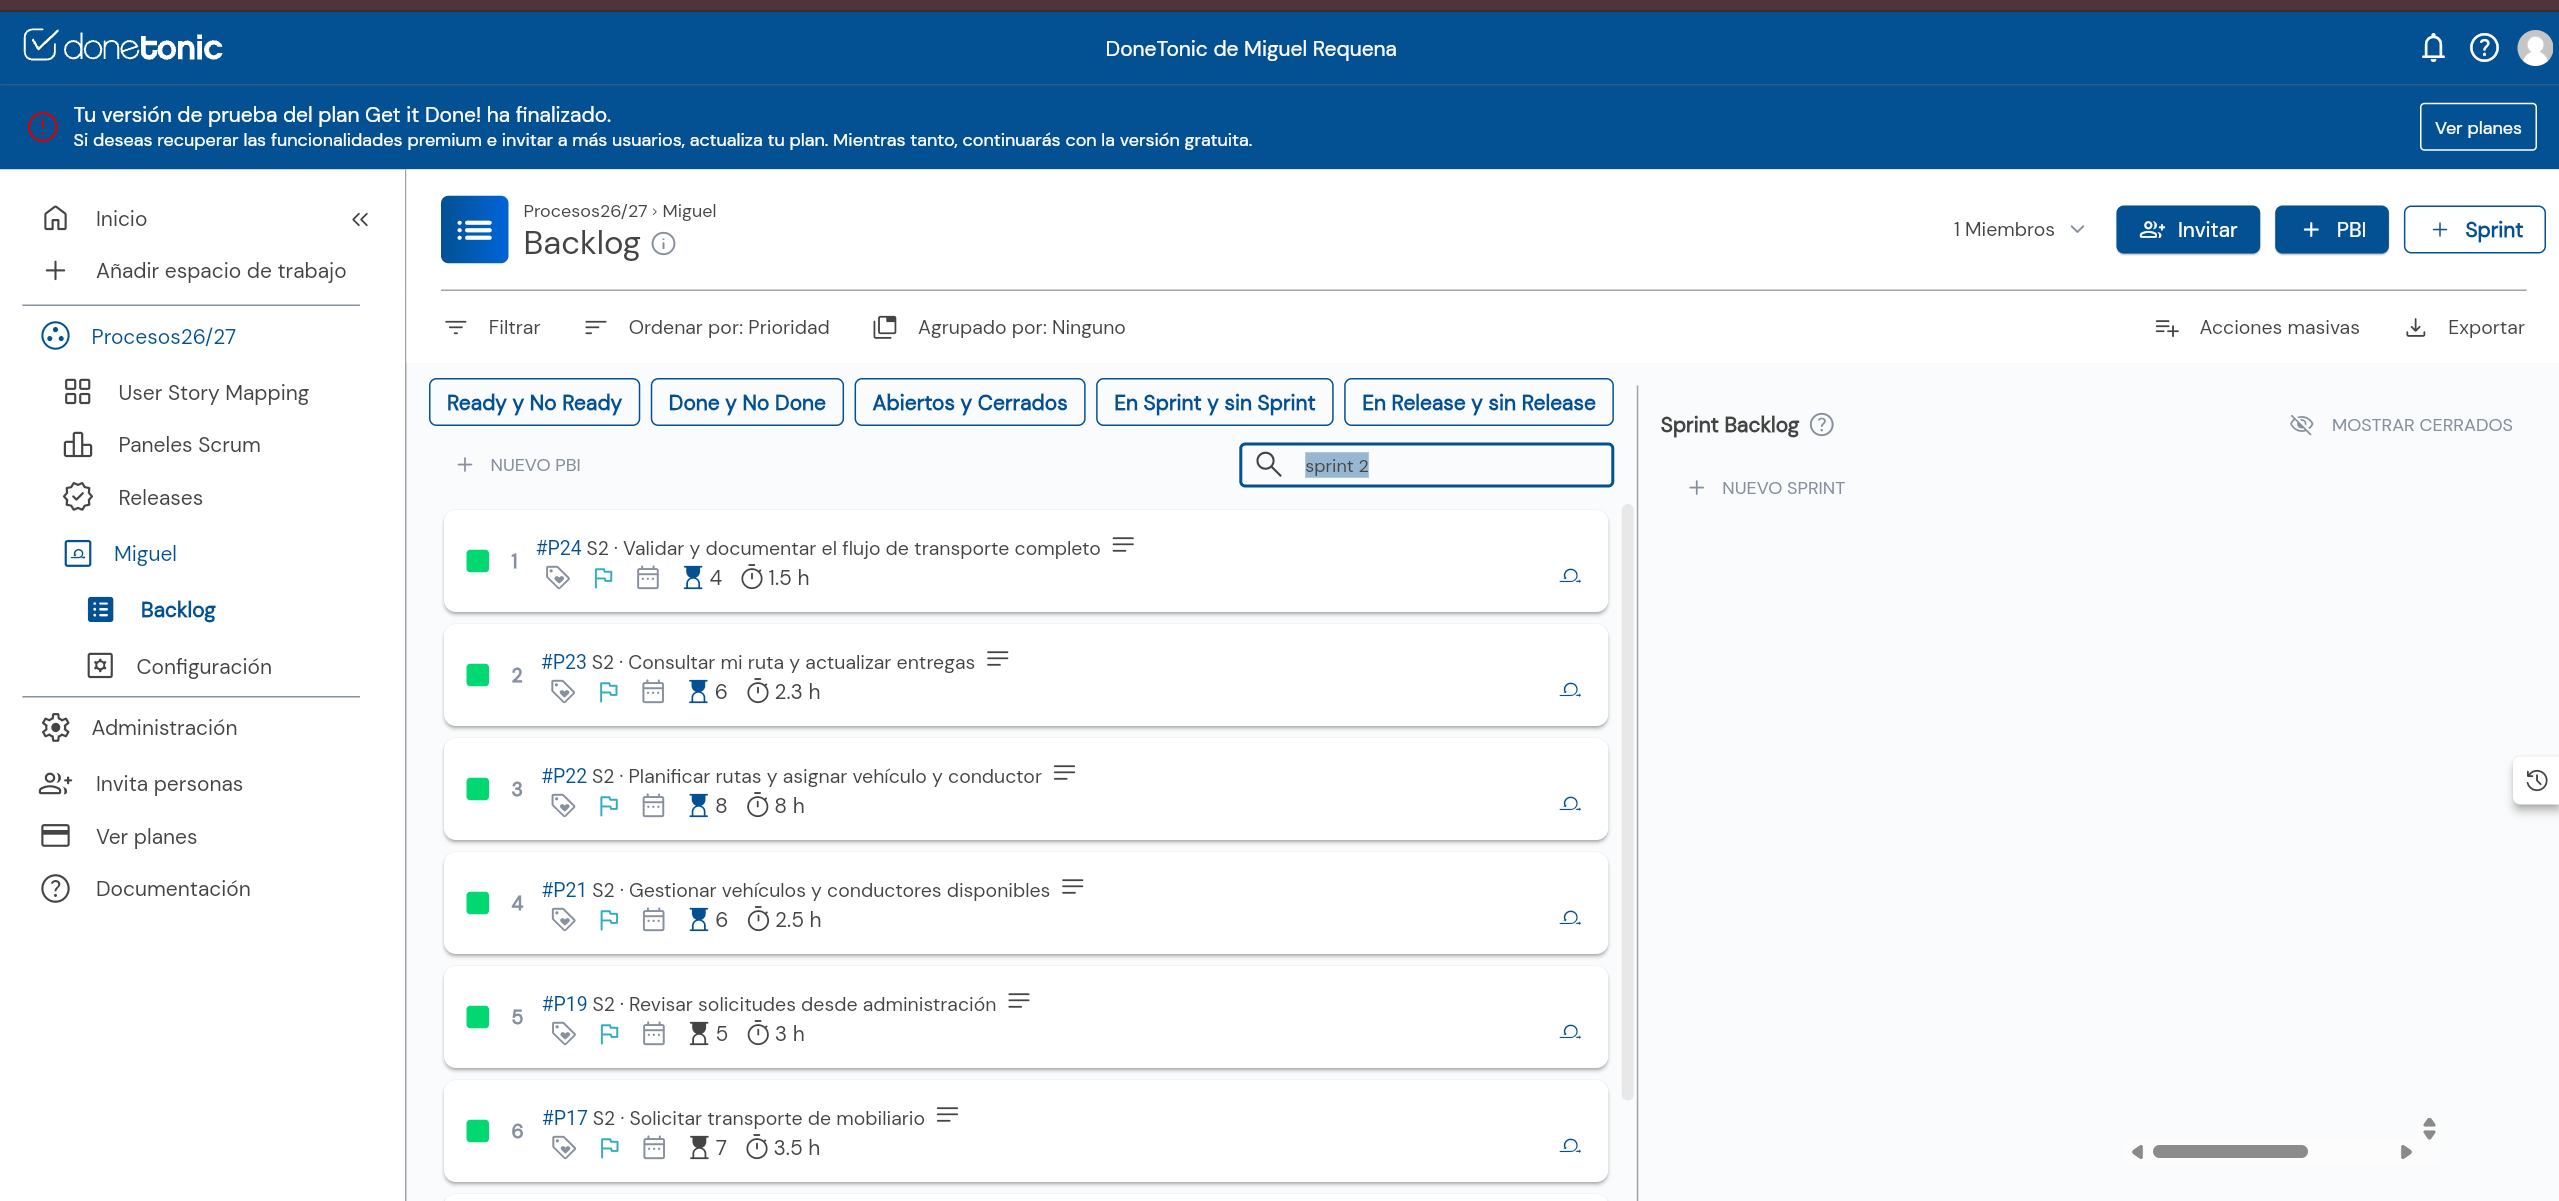
\includegraphics[width=0.95\textwidth,height=0.43\textheight,keepaspectratio,trim=215bp 0bp 469bp 250bp,clip]{figs/donetonic-sprint2-backlog.png}
\captionsetup{hypcap=false}
\captionof{figure}{Recorte de la vista parcial del backlog del Sprint 2 aportada el 17 de noviembre: P24, P23, P22, P21, P19 y P17, con estimaciones y horas registradas.}
\label{fig:s2-backlog}
\end{minipage}
\end{center}
\begin{center}
\begin{minipage}{\textwidth}
\centering
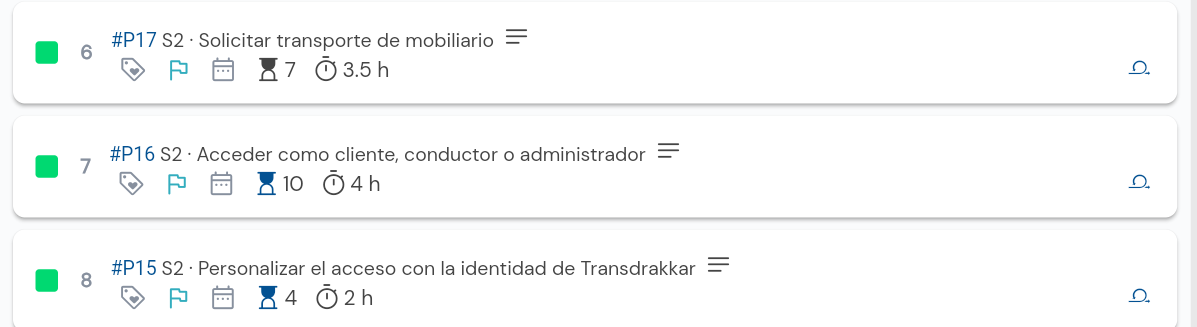
\includegraphics[width=0.95\textwidth,height=0.28\textheight,keepaspectratio]{figs/donetonic-sprint2-backlog-resto.png}
\captionsetup{hypcap=false}
\captionof{figure}{Continuación del backlog: P17, P16 y P15. P17 aparece en ambas capturas y solo se cuenta una vez.}
\label{fig:s2-backlog-resto}
\end{minipage}
\end{center}

\subsection{Validación del incremento}
El PR 42 integra la revisión de cierre \texttt{885b380}. La ejecución de GitHub Actions del PR, identificada por el número \texttt{44078563639}, contiene 85 casos, sin fallos ni omisiones, con MongoDB real configurado como replica set. También se construyó y comprobó el contenedor. El informe JUnit queda como artefacto descargable de esa ejecución. La regresión local contiene 83 casos superados y dos integraciones MongoDB omitidas por falta de una instancia local; no se presentan esas omisiones como pruebas superadas.

El escenario T34 recorre por HTTP alta de solicitud, aceptación, recursos, ruta, incidencia, resolución y consulta del cliente. Se recuperan sesión, detalle e itinerario completado en otro proceso. Las pruebas MongoDB comprueban transacciones, rollback, reintentos simultáneos, conflictos y liberación de reservas. T35 añade permisos, fechas inválidas, duplicados, transiciones no autorizadas y fallos de red. La revisión visual utiliza dos paradas ficticias y comprueba el motivo obligatorio, las dos entregas y su historial desde el perfil cliente.

La revisión desplegada sirve la nueva interfaz de entregas y mantiene el endpoint operativo protegido: una petición sin sesión devuelve 401. No se modificaron datos de transporte reales para demostrar el cierre. La revisión funcional no acredita recepción real de correo, consentimiento Google ni un reinicio manual de Cloud Run.

\subsection{Retrospectiva y gráficos de seguimiento}
El burndown de la Figura~\ref{fig:s2-burndown} parte de 57 unidades de estimación, muestra aproximadamente 43 pendientes en el día 12 y alcanza cero en el día 21. La reducción se concentra en el tramo final. Esa forma describe el registro de cierres, pero no demuestra que todo el trabajo se realizase en esos últimos días. Una mejora del proceso consiste en registrar los cierres y tiempos al terminar cada tarea.
\begin{center}
\begin{minipage}{\textwidth}
\centering
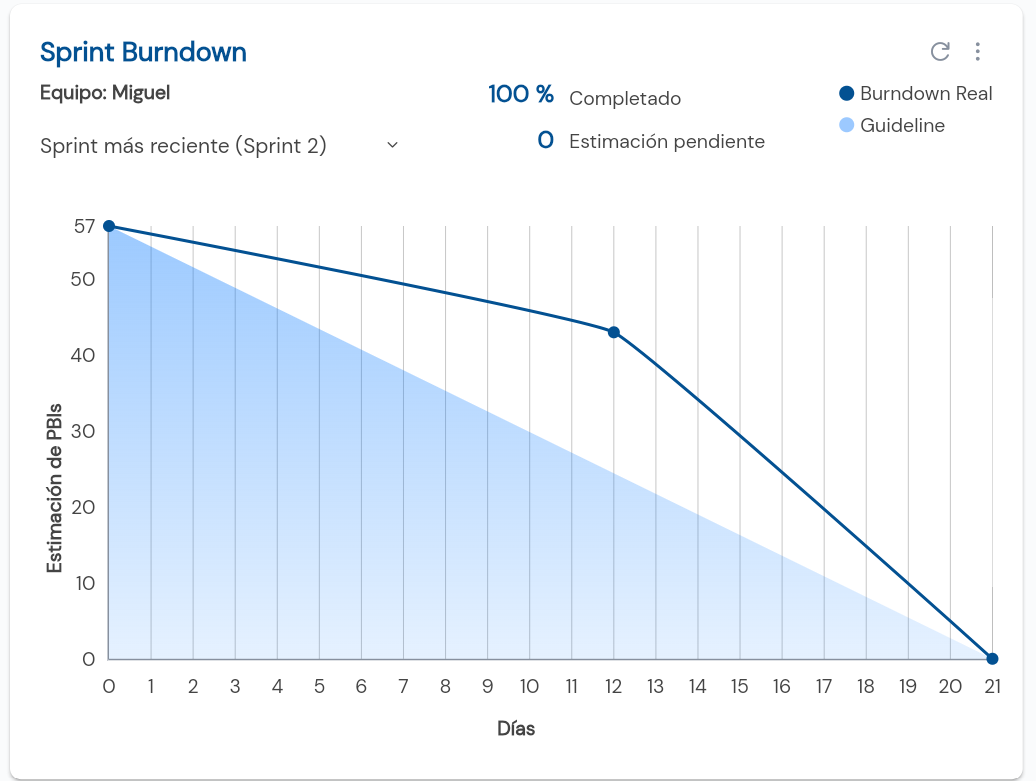
\includegraphics[width=0.95\textwidth,height=0.58\textheight,keepaspectratio]{figs/donetonic-sprint2-burndown.png}
\captionsetup{hypcap=false}
\captionof{figure}{Burndown del Sprint 2: 100\% completado, cero estimación pendiente y final en el día 21. La unidad del eje vertical es la estimación de PBI mostrada por DoneTonic.}
\label{fig:s2-burndown}
\end{minipage}
\end{center}

El burnup de la Figura~\ref{fig:s2-burnup} muestra aproximadamente 14 unidades completadas en el día 12 y 57 en el día 21. La línea discontinua denominada Trabajo Total se mantiene alrededor de 9 después del día 7, sin coincidir con el final de 57 de la serie real. Además, la suma de estimaciones de los ocho PBI transcritos es 50. Las capturas no permiten determinar la causa de estas diferencias de agregado o configuración. Por ello, se conservan las figuras originales y no se fuerza una conciliación ni se equiparan esos valores a horas. El indicador 100\% y el pendiente cero se interpretan como estado comunicado por la herramienta, no como explicación de su cálculo.
\begin{center}
\begin{minipage}{\textwidth}
\centering
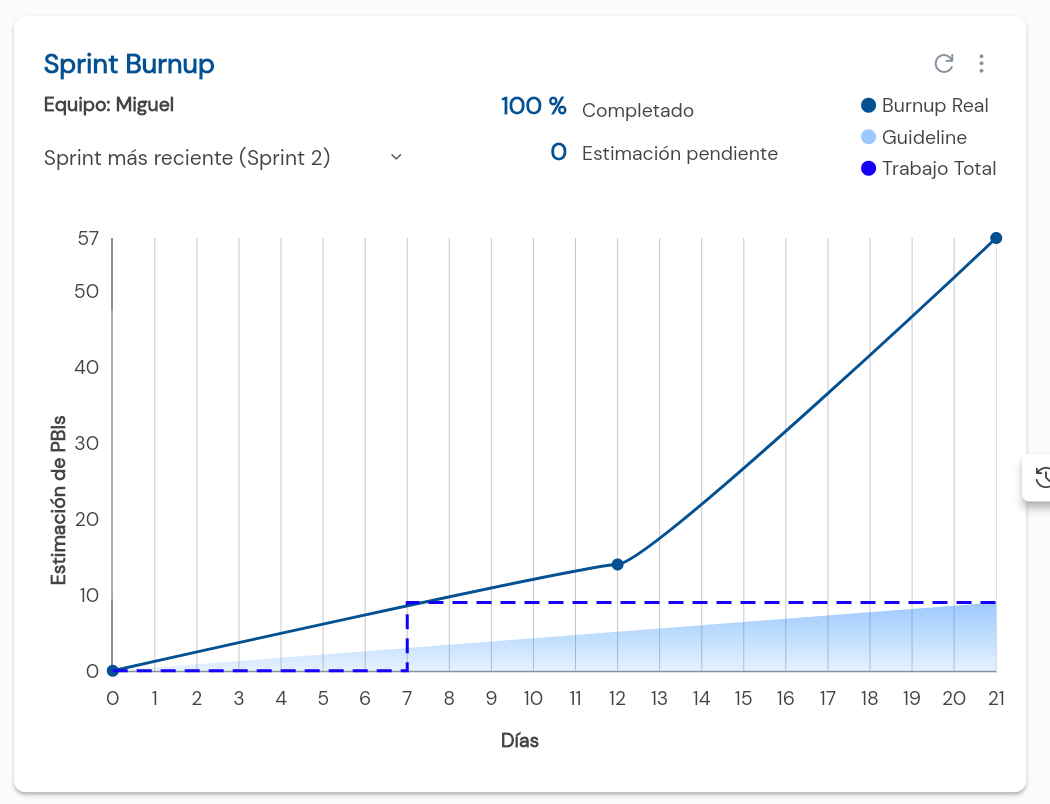
\includegraphics[width=0.95\textwidth,height=0.58\textheight,keepaspectratio]{figs/donetonic-sprint2-burnup.png}
\captionsetup{hypcap=false}
\captionof{figure}{Burnup del Sprint 2. Se conserva la discrepancia visible entre la serie real, Trabajo Total y la suma de estimaciones de los PBI, sin corregir ni reconstruir el gráfico.}
\label{fig:s2-burnup}
\end{minipage}
\end{center}

Como resultado positivo, el sprint entrega un flujo de transporte completo con separación de perfiles, historial y consistencia transaccional. Las incidencias de solicitudes antiguas incompletas y los conflictos de planificación se tradujeron en validaciones y mensajes concretos. La principal mejora de seguimiento es mantener alineados backlog y gráficos y registrar el esfuerzo con la misma fecha de corte. Se recomienda revisar la configuración de los agregados de DoneTonic antes de utilizar sus gráficos para comparar productividad o variación de alcance.
